\documentclass{article}
\usepackage[utf8]{inputenc}
\usepackage[spanish]{babel}
\usepackage{natbib}
\usepackage{graphicx}
\usepackage{mathtools}
\usepackage{color}
\usepackage{float}
\usepackage{fancyhdr}
\usepackage{adjustbox}
\usepackage{pdflscape}
\usepackage{verbatim}

\pagestyle{fancy}
\lhead{Grupo 4 - Turno 7}
\chead{Trabajo Practico Nro 1}
\rhead{Primer Cuatrimestre 2015}


\begin{document}

\section{Objetivo}
Analizar problemas electrostáticos, calcular el campo eléctrico y la función potencial en distintos puntos del espacio.

\section{Desarrollo}
\subsection{Ejercicio 1}
Una distribución cilíndrica de carga, denominada “cilindro 1”, cargada sobre la superficie. El radio (R) de la distribución es de 2cm y la carga está dada por $ \sigma = +1 \mu C/m^2 $.
Se considera que el diámetro del cilindro es mucho menor a las distancias involucradas.

\begin{figure}[H]
\centering
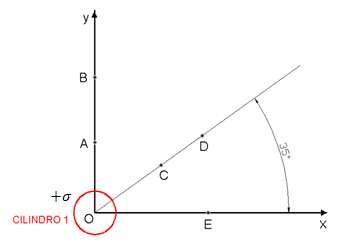
\includegraphics[scale=1]{1.png}
\caption{Esquema (fuera de escala)}
\label{fig:1}
\end{figure}

\subsubsection{Campo eléctrico}

\begin{comment}
Para $r<R$
	\begin{equation}
			\overrightarrow{E} = 0
	\end{equation}

Para $r>R$
\end{comment}

En función de una densidad lineal de carga.
	\begin{equation}
		E_x = \frac{\lambda x}{2 \pi \varepsilon_0 (x^2 + y^2)}
	\end{equation}

	\begin{equation}
		E_y = \frac{\lambda y}{2 \pi \varepsilon_0 (x^2 + y^2)}
	\end{equation}

    \begin{equation}
		E_z = 0
	\end{equation}

En función de una densidad superficial de carga.
	\begin{equation}
    	E_x = \frac{\sigma Rx}{\varepsilon_0 (x^2 + y^2)}
    \end{equation}

	\begin{equation}
		E_y = \frac{\sigma Ry}{\varepsilon_0 (x^2 + y^2)}
	\end{equation}

    \begin{equation}
		E_z = 0
	\end{equation}
    
\subsubsection{Función Potencial}

\begin{comment}
Para $r<R$:
	\begin{equation}
		V(r) = \frac{\lambda}{2 \pi \varepsilon_0}\ln \left(\frac{C}{R}\right)
	\end{equation}
    
    Para $r>R$:
\end{comment}

\begin{equation}
		V(r) = \frac{\lambda}{2 \pi \varepsilon_0}\ln \left(\frac{C}{\sqrt[]{x^2 + y^2}}\right)
	\end{equation}

\subsubsection{Resultados}
	\begin{table}[H]
    \centering
    \begin{tabular}{|l | c | r|}
    	\hline
		Punto & Distancia (cm) & $ \varphi $ \\ \hline
        OA & 12 & 90 \\
        OB & 32 & 90 \\
        OC & 12 & 35 \\
        OD & 22 & 35 \\
        OE & 19 & 0 \\ \hline
	\end{tabular}
    \caption{Datos}
    \end{table}
    
    \begin{table}[H]
	\centering
	\begin{tabular}{|l | c | c | r|}
    	\hline
        Punto & $\overrightarrow{E} (V/m)$ & $|E| (V/m)$ &Potencial (V) \\ \hline
        OA & $ 18832,4 \hat{i} $ & 18832,4 & 0 \\
        OB & $ 7062,15 \hat{j} $ & 7062,15 & -2216,6 \\
        OC & $ 15430,8 \hat{i} +  10799,99 \hat{j} $ & 18834,8 & 0 \\
        OD & $ 8426,13 \hat{i} +  5898,29 \hat{j} $ & 10285,4 & -1369,8\\
        OE & $ 11894,14 \hat{i} $ & 11894,14 & -1038,5\\ \hline
	\end{tabular}
    \caption{Resultados analíticos}
    \end{table}
    
    \begin{table}[H]
	\centering
	\begin{tabular}{|l | r|}
    	\hline
        Punto & Potencial (V) \\ \hline
        OA & 0  \\  %este valor esta dibujado 
        OB & -2278,4 \\ 
        OC & 0 \\ 
        OD & -1402,4 \\ 
        OE & -1084,3 \\ \hline %este valor esta dibujado
	\end{tabular}
    \caption{Resultados obtenidos con el femm}
    \end{table}
    
         \begin{table}[H]
	\centering
	\begin{tabular}{|l | r|}
    	\hline
        Punto & $\varepsilon de Potencial$\\ \hline
        OA & 0 \%\\
        OB & 2,8 \% \\
        OC & 0 \%\\
        OD & 2,4 \%\\
        OE & 4,4 \%\\ \hline
	\end{tabular}
    \caption{Errores porcentuales entre los resultados analíticos y numéricos}
    \end{table}
    
    \begin{comment}
    \begin{table}[H]
    \centering
  
    \begin{tabular}{|l | c | c | c | c | c | c | c | r|}
		\hline
        Punto & $E_x$ (N/C) & $E_y$ (N/C) & $E$ (N/C) & Potencial (V) & $E_x$ (N/C) FEMM & $E_y$ (N/C) FEMM & $E$ (N/C) FEMM & Potencial (V) FEMM\\ \hline
        OA & 0 & 188832,4 & completar & 0 & completar & completar & completar & completar \\
        OB & 0 & 7062,15 & completar & -2216,6 & completar & completar & completar & completar \\
        OC & completar & completar & completar & 0 & completar & completar & completar & completar \\
        OD & completar & completar & completar & -1369,8 & completar & completar & completar & completar \\
        OE & 11199,76 & 0 & completar & completar & completar & completar & completar & completar \\ \hline
	\end{tabular}
    \caption{Resultados}
    \end{table}
    \end{comment}
    
\begin{comment}
	\begin{table}[H]
    \centering
    \begin{tabular}{|l | c | r|}
		\hline
        Punto & Campo Eléctrico (N/C)& Potencial (V) \\ \hline
        OA & $8726,81 \hat{i} + 132279,10 \hat{j}$ & 3463,37 \\
        OB & $1628,91 \hat{i} + 3010,11 \hat{j}$ & 2278,42 \\
        OC & $94642,20 \hat{i} - 6099,99 \hat{j}$ & 0 \\
        OD & $-1257,57 \hat{i} - 459,96 \hat{j}$ & 1966,92 \\
        OE & $4328,39 \hat{i} + 5908,17 \hat{j}$ & 2468,32 \\ \hline
	\end{tabular}
    \caption{Resultados obtenidos con el femm}
    \end{table}
\end{comment}

\subsection{Ejercicio 2}
Dos distribuciones cilíndricas superficiales de carga de distinto signo, separadas una cierta distancia “d”, denominadas “cilindro 1” y “cilindro 2”. 
El radio (R) de cada distribución cilíndrica es de 2cm y la densidad de cargas superficial es $ \sigma = \pm 1 \mu C/m^2 $. 
“Cilindro 1” se encuentra en el origen de coordenadas y es el de densidad de carga positiva. 
Se considera que los diámetros de los cilindros son mucho menores que las distancias involucradas.

\begin{figure}[H]
	\centering
	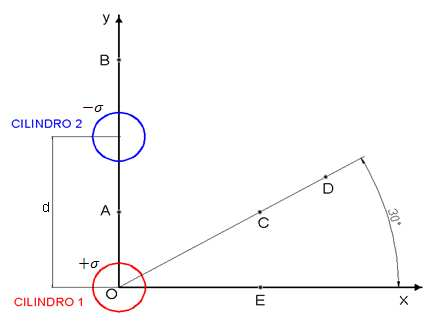
\includegraphics[scale=1]{2.png}
	\caption{Esquema (fuera de escala)}
	\label{fig:2}
\end{figure}

\subsubsection{Campo eléctrico}
    Campo fuera de ambos cilindros.\\

En función de una densidad lineal de carga.
	
    \begin{equation}
    	E_x = \frac{\lambda x}{2 \pi \varepsilon_0} \left(\frac{1}{x^2 + y^2} - \frac{1}{x^2 + (y-d)^2}\right)  
    \end{equation}

	\begin{equation}
		E_y = \frac{\lambda}{2 \pi \varepsilon_0} \left(\frac{y}{x^2 + y^2} - \frac{y-d}{x^2 + (y-d)^2}\right)
	\end{equation}

    \begin{equation}
		E_z = 0
	\end{equation}

En función de una densidad superficial de carga.
	    
    \begin{equation}
    	E_x = \frac{\sigma Rx}{\varepsilon_0} \left(\frac{1}{x^2 + y^2} - 
        \frac{1}{x^2 + (y-d)^2}\right)  
    \end{equation}

	\begin{equation}
		E_y = \frac{\sigma R}{\varepsilon_0} \left(\frac{y}{x^2 + y^2} - 
        \frac{y-d}{x^2 + (y-d)^2}\right)
	\end{equation}
    
    \begin{equation}
		E_z = 0
	\end{equation}
    
\begin{comment}
    Campo dentro del cilindro 1.
    \begin{equation}
    	E_x = \frac{\sigma Rx}{\varepsilon_0 (x^2 + (y-d)^2)}
    \end{equation}
	
    \begin{equation}
    	E_y = \frac{\sigma R(y-d)}{\varepsilon_0 (x^2 + (y-d)^2)}
    \end{equation}

	\begin{equation}
		E_z = 0
	\end{equation}
	
    Campo dentro del cilindro 2.

	\begin{equation}
    	E_x = \frac{\sigma Rx}{\varepsilon_0 (x^2 + y^2)}
    \end{equation}
	
    \begin{equation}
    	E_y = \frac{\sigma Ry}{\varepsilon_0 (x^2 + y^2)}
    \end{equation}

	\begin{equation}
		E_z = 0
	\end{equation}    
\end{comment}

\subsubsection{Función Potencial} 
	
    \begin{equation}
		V(r) = V_1(r) + V_2(r)	
    \end{equation}
    
    Calculo del potencial total. $V_1$ y $V_2$ son los potenciales dentro de los cilindros 1 y 
    2 respectivamente.
    
	\begin{equation}
    	V_1(r) = \frac{\lambda}{2 \varepsilon_0 \pi}\ln \left({\frac{c}{\sqrt[]{x^2 + y^2}}}\right)
    \end{equation}
    
    \begin{equation}
		V_2(r) = \frac{\lambda}{2 \varepsilon_0 \pi}\ln \left({\frac{\sqrt[]{x^2 + (y-d)^2}}{c}}\right)
	\end{equation}
    
    Sabiendo que $ r' = r - d$ y que $\sigma = 
    \frac{\lambda}{2 \pi R}$:
    \begin{equation}
		V(r) = \frac{\lambda}{2 \varepsilon_0 \pi} \ln \left({\sqrt[]{\frac{x^2 + (y-d)^2}{x^2 + y^2}}}\right)
	\end{equation}
    

\subsubsection{Resultados}
	\begin{table}[H]
    \centering
    \begin{tabular}{|l | c | r|}
    	\hline
		Punto & Distancia ($cm$) & $ \varphi $ \\ \hline
        d & 34 & - \\
        OA & 17 & 90 \\
        OB & 64 & 90 \\
        OC & 34 & 30 \\
        OD & 49 & 30 \\
        OE & 52 & 0 \\ \hline
	\end{tabular}
    \caption{Datos}
    \end{table}

	\begin{comment}
    \begin{table}[H]
    \begin{adjustbox}{max width=\columnwidth}
    \centering
    \begin{tabular}{|l | c | c | c | c | c | c | c | r|}
		\hline
        Punto & $E_x$ (N/C) & $E_y$ (N/C) & $E$ (N/C) & Potencial (V) & $E_x$ (N/C) FEMM & $E_y$ (N/C) FEMM & $E$ (N/C) FEMM & Potencial (V) FEMM\\ \hline
        OA & completar & completar & completar & 0 & completar & completar & completar & completar \\
        OB & completar & completar & completar & completar & completar & completar & completar & completar \\
        OC & completar & completar & completar & 0 & completar & completar & completar & completar \\
        OD & completar & completar & completar & completar & completar & completar & completar & completar \\
        OE & completar & completar & completar & 476,8 & completar & completar & completar & completar \\ \hline
	\end{tabular}
    \end{adjustbox}
    \caption{Resultados}
    \end{table}
    \end{comment}
	
    \begin{table}[H]
	\centering
	\begin{tabular}{|l | c | c | r|}
    	\hline
        Punto & $\overrightarrow{E} (V/m)$ & $|E| (V/m)$ &Potencial (V) \\ \hline
        OA & $26586,9\hat{j} $ & 26586,9 & 0 \\
        OB & $ - 4001,9 \hat{j}$ & 4001,9 & -1712,3 \\
        OC & $ 6661,9 \hat{j}$ & 6661,9 & 0 \\
        OD & $-1079,5 \hat{i} +  3446,7 \hat{j}$ & 3611,8 &-270,2 \\
        OE & $ 1300,9 \hat{i} + 1990,6 \hat{j}$ & 2378,0 &402,2 \\ \hline
	\end{tabular}
    \caption{Resultados analíticos}
    \end{table}

    \begin{table}[H]
	\centering
	\begin{tabular}{|l | c | c | r |}
    	\hline
        Punto & $\overrightarrow{E} (V/m)$ & $|E| (V/m)$ & Potencial (V) \\ \hline
        OA & $142,6 \hat{i} + 26415,8 \hat{j}$ & 26415,8 & -1,4 \\
        OB & $-62,2 \hat{i} - 3989,1 \hat{j}$ & 3989,5 & -1740,4 \\
        OC & $74,3 \hat{i} + 7386,5 \hat{j}$ & 7386,9 & 0 \\
        OD & $-1086,8 \hat{i} + 3502,3 \hat{j}$ & 3667,0 & -274,3 \\
        OE & $1314,1 \hat{i} + 2008,1 \hat{j}$ & 2399.8 & 409,7 \\ \hline
	\end{tabular}
    \caption{Resultados obtenidos con el femm}
    \end{table}
    
     \begin{table}[H]
	\centering
	\begin{tabular}{|l | c | r |}
    	\hline
        Punto & $\varepsilon de |E|$ & $\varepsilon de Potencial$\\ \hline
        OA & 0,6\% & 1\%\\
        OB & 0,3\% & 1,6\% \\
        OC & 10\% & 0\%\\
        OD & 1,5\% & 1,5\%\\
        OE & 0,9\% & 1,9\%\\ \hline
	\end{tabular}
    \caption{Errores porcentuales entre los resultados analíticos y numéricos}
    \end{table}


\section{Conclusiones}

A continuación, presentamos una serie de conclusiones obtenidas a partir del desarrollo del trabajo:
\begin{itemize}
		\item Es posible el paso de una densidad superficial de carga, a una densidad lineal, si tenemos en cuenta que la superficie se puede pensar como un conjunto infinito de hilos unidos.Se pueden expresar una en función de la otra.
		\item Al igual que con los campos eléctricos, el principio de superposición se puede aplicar para calcular el potencial, en el caso de los dos cilindros.
		\item Si logramos hacer una simulación lo suficientemente cercana al modelo ideal, en el caso 1 (un cilindro) el error porcentual puede llegar a ser nulo o, si no lo es, su valor es menor al 5\%. Es decir, las simulaciones correctamente planteadas se acercan de forma considerable a los resultados y modelos ideales.
        \item En el segundo caso (dos cilindros), una simulación correctamente realizada, nos da solo un 2\% de error respecto a los valores ideales calculados con las fórmulas obtenidas. Es un caso mucho más cercano a ideal, que el primero.
        

	\end{itemize}

\end{document}